\section{模型建立与求解}
\label{sec:model}

\subsection{符号约定与四问递进的总体设计}
\label{sec:framework}

本文四问构成一条递进主线：问题一刻画数据本身的质量与配比，问题二把数据因素纳入标度律，问题三在算力预算下求解最优配置，问题四用历史评测数据检验规律并预测能力前沿。前一问的输出是后一问的输入，统一符号如下。

\begin{table}[htbp]
  \centering
  \caption{全文主要符号与四问接口}
  \label{tab:symbols}
  \renewcommand{\arraystretch}{1.2}
  \begin{tabular}{lll}
    \toprule
    符号 & 含义 & 产生方 $\to$ 使用方 \\
    \midrule
    $Q_i$ & 样本级质量分数（TOPSIS，$0$--$100$） & 问题一 $\to$ 聚合为 $Q_g$ \\
    $Q_g$ & 领域级质量评分（7 个质量域） & 问题一 $\to$ 经 A16 映射进入问题二、三 \\
    $p$ & 17 域训练配比（单纯形约束） & 问题一 $\to$ 问题二、三的决策/条件变量 \\
    $N,D$ & 参数量、训练数据量（十亿单位） & 附件 B $\to$ 问题二、三 \\
    $L$ & 验证集交叉熵损失 & 各问统一的可观测目标 \\
    $E,\alpha,\beta$ & 标度律参数（本文自行估计，不用任何预置值） & 问题二 $\to$ 问题三 \\
    $\varepsilon_N,\varepsilon_D,\varepsilon_Q$ & 各因素弹性 & 问题二 $\to$ 问题三的成本—收益比较 \\
    $C$ & 总算力预算（FLOPs） & 问题三（$C=6ND+\Delta C_Q+\Delta C_S$） \\
    $S$ & 上下文长度（外生，取值依据 C7） & 问题三 \\
    \bottomrule
  \end{tabular}
\end{table}

接口设计的三条原则。其一，\emph{质量与配比经问题一引入}：问题二、三不重复读取质量信号原始文件，而是使用问题一输出的 $Q_g$ 与配比模型；质量域（7 个）与配方域（17 个）口径不同，跨体系关联采用附件 A16 的参考映射并声明假设。其二，\emph{损失是唯一跨附件的可观测桥梁}：附件 A、B 实验相互独立，但均以交叉熵损失为输出，本文以损失为统一因变量建立可检验的衔接假设；附件 C 提供 Loss--Benchmark 桥接（C6），用于问题四把“扣分”翻译为“评测得分”。其三，\emph{半合成数据分层使用}：Cerebras 轨迹（B2）、NQ 实验（B6--B8）为真实数据校准的半合成补充，只用于补充分析与敏感性讨论，不作为直接实验观测，全部相关结论在文中显式标注。

以下依次给出问题一的三项建模：质量评价（第~\ref{sec:q1-quality}~节）、质量冲突消解（第~\ref{sec:q1-conflict}~节）、领域配比建模（第~\ref{sec:q1-mixture}~节）。

% 问题一·第一小问：数据质量评价（正式章节）
% 由 sections/drafts/q1-quality-evaluation.tex 清洗接入：去除草稿头注、描述统计统一为两位小数。
% 数据来源：run q1-critic-topsis-20260924-r01；主张见 paper/claim-ledger.csv（Q1-WPB-*）。
\subsection{问题一：数据质量评价、质量冲突消解与领域配比建模}
\label{sec:q1}

\subsubsection{第一小问：数据质量评价}
\label{sec:q1-quality}

\paragraph{问题分析与总体框架}
本小问的目标是将抽样集与扩展集中的多源文本质量信号统一到同一评价尺度，形成可解释、可追溯的质量分数。评价对象包括抽样集 $A_1$、扩展集 $A_2$ 和扩展集 $A_3$ 的全部记录：$A_1$ 含 $51{,}230$ 条，$A_2$ 含 $17{,}523$ 条，$A_3$ 含 $203{,}752$ 条。合并后按记录指纹去重：$272{,}505$ 条文件记录中 $11{,}419$ 条为跨集重复，得到 $261{,}086$ 条唯一记录。模型流程为“全量合并与去重—指标方向统一—稳健归一化—CRITIC 客观赋权—加权距离 TOPSIS 评分—样本、领域和语料级聚合—抽样集对照”。

\begin{figure}[htbp]
  \centering
  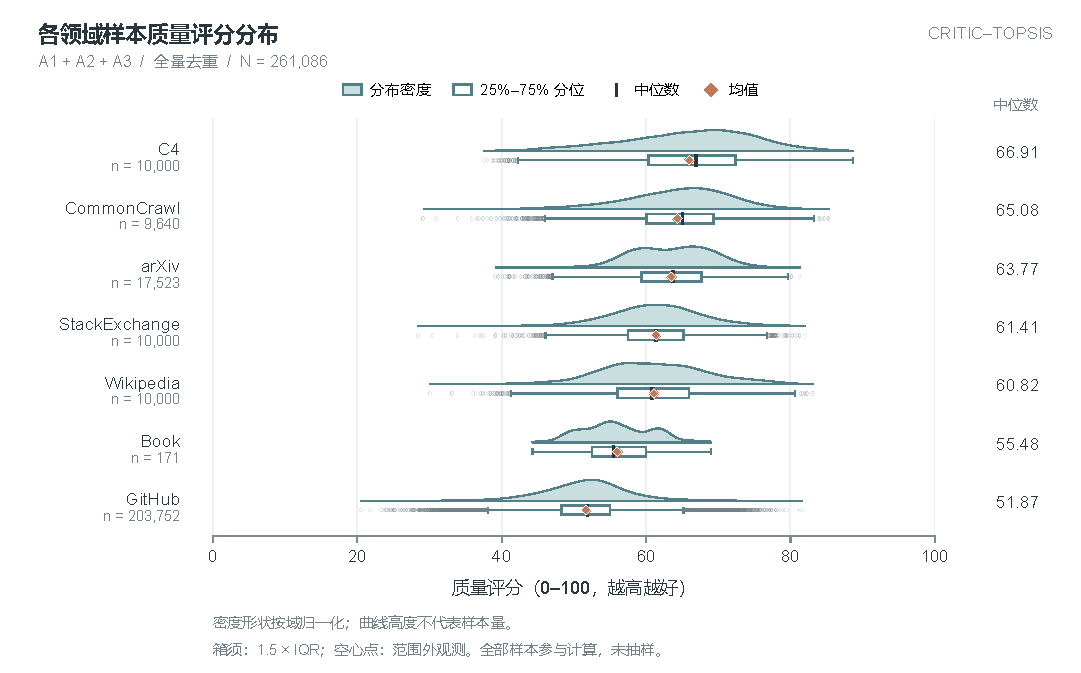
\includegraphics[width=\linewidth]{figures/q1-critic-topsis/nature-v1/figure01_domain_distribution_nature.pdf}
  \caption{全量去重语料的领域构成及抽样集对照。柱形表示各领域记录数，折线表示领域在全量语料中的占比；阴影区域标示扩展集带来的组成变化。}
  \label{fig:q1-nature-01}
\end{figure}

\paragraph{数据对象与预处理}
设第 $i$ 条记录的原始质量指标向量为 $\boldsymbol{x}_i=(x_{i1},\ldots,x_{i16})$。16 个指标覆盖语言形式、可读性、内容质量、教育性、事实性、知识覆盖与重复性等维度，其中句末标点率、cleanliness、no-ad、readability、fluency、unique words、QuRating education、writing、FineWeb education、factual、Books、Math 和 Wikipedia 为正向指标；无字母词比例、最高频二元词组占比和最高频三元词组占比为负向指标。负向指标取值较大通常意味着文本更可能由符号、模板或高频短语主导，故按噪声与重复性的代理假设作反向处理。

记方向统一后的指标为
\begin{equation}
 \widetilde{x}_{ij}=\begin{cases}
 x_{ij}, & j\in\mathcal{P},\\
 -x_{ij}, & j\in\mathcal{N},
 \end{cases}
 \qquad \mathcal{P}\cup\mathcal{N}=\{1,\ldots,16\},\quad \mathcal{P}\cap\mathcal{N}=\varnothing,
 \label{eq:q1-direction-unification}
\end{equation}
其中 $\mathcal{P}$ 和 $\mathcal{N}$ 分别为正向、负向指标集合。随后以 $A_1$ 拟合集上方向统一值的 $1\%$ 和 $99\%$ 分位数作为稳健边界 $l_j$、$u_j$，统一为“越高越好”的归一化形式
\begin{equation}
 z_{ij}=\operatorname{clip}\left(\frac{\widetilde{x}_{ij}-l_j}{u_j-l_j},0,1\right),
 \qquad
 \operatorname{clip}(t,0,1)=\min\{1,\max\{0,t\}\}.
 \label{eq:q1-robust-normalization}
\end{equation}
$A_1$ 按记录 ID 的固定哈希规则划分为 40,919 条拟合集与 10,311 条留出集；归一化边界与下文权重仅由拟合集估计，留出集及 $A_2$、$A_3$ 均不重新拟合，从而保证各集合分数可比。归一化后检查缺失值、无穷值、越界值和重复指纹，并保留每条记录的来源集、领域标签和质量分数，供后续聚合与审计。

\begin{figure}[htbp]
  \centering
  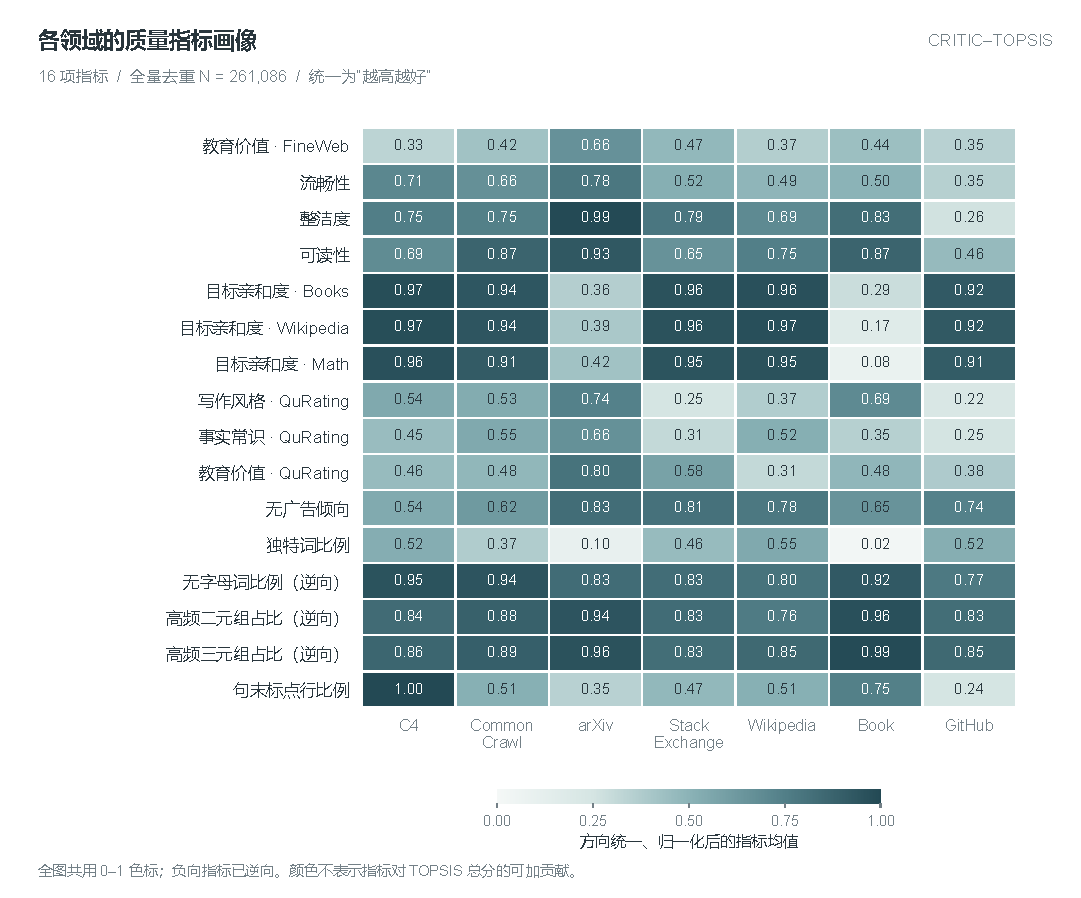
\includegraphics[width=\linewidth]{figures/q1-critic-topsis/nature-v1/figure02_indicator_heatmap_nature.pdf}
  \caption{16 个质量指标的方向统一、归一化分布及指标间相关性。颜色表示归一化后的指标水平；右侧标注负向指标在方向统一后的含义。}
  \label{fig:q1-nature-02}
\end{figure}

\paragraph{CRITIC 客观赋权}
为避免人为指定权重，采用 CRITIC 方法同时利用指标的离散程度和冲突程度。设归一化矩阵为 $Z=(z_{ij})$，第 $j$ 个指标的样本标准差为 $\sigma_j$，与第 $k$ 个指标的 Pearson 相关系数为 $r_{jk}$，则信息量为
\begin{equation}
 I_j=\sigma_j\sum_{k=1}^{16}(1-r_{jk}),\qquad
 w_j=\frac{I_j}{\sum_{m=1}^{16}I_m},\qquad
 \sum_{j=1}^{16}w_j=1.
 \label{eq:q1-critic}
\end{equation}
其中 $\sigma_j$ 反映指标对样本的区分能力，$1-r_{jk}$ 反映该指标与其他指标的信息冗余程度。权重由 $A_1$ 拟合集计算并固定用于留出集及 $A_2$、$A_3$。最终权重最高的三个指标为句末标点率（$8.91\%$）、cleanliness（$8.00\%$）和 no-ad（$7.75\%$）；三个负向词组指标合计权重为 $16.58\%$。需要说明的是，句末标点率等格式性指标权重居前，反映的是 CRITIC 以离散度与冗余度赋权的机制特征，即哪怕这些指标在样本间变异大、与其他指标冗余低，也无法证明格式特征比语义特征“更重要”；这一点在敏感性分析（图~\ref{fig:q1-nature-06}）中进一步检验。

\begin{figure}[htbp]
  \centering
  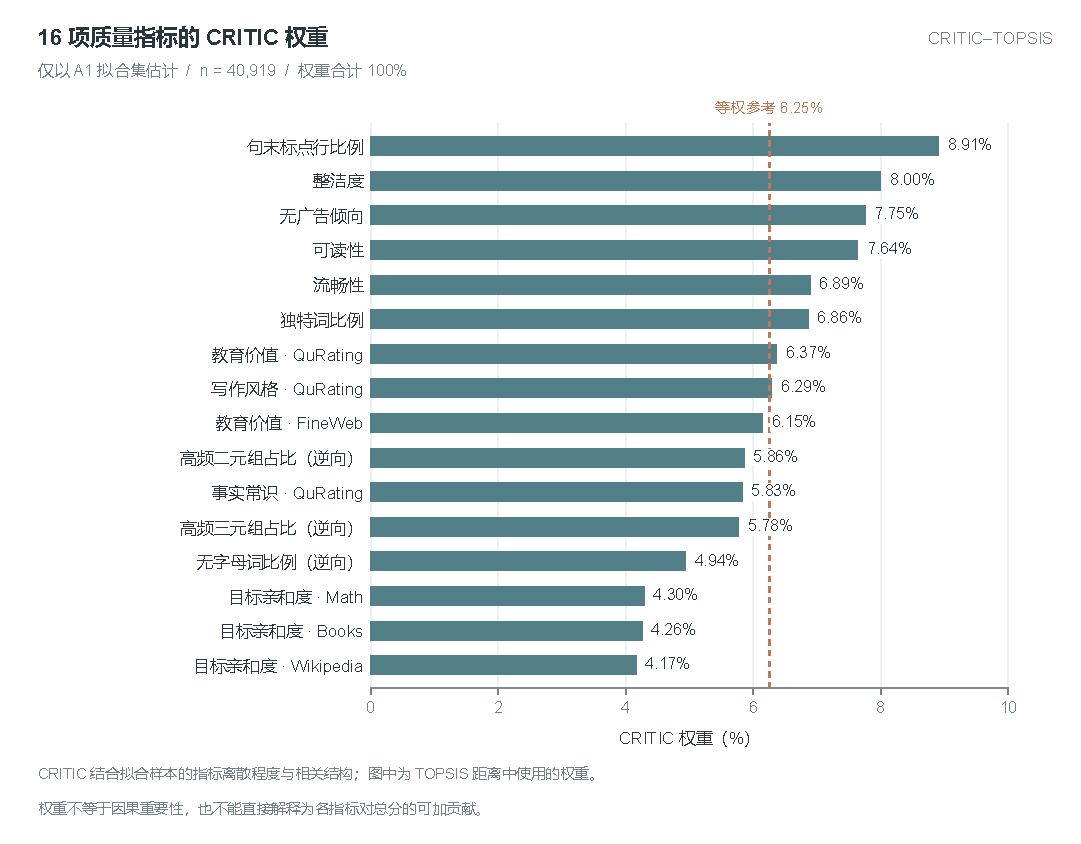
\includegraphics[width=\linewidth]{figures/q1-critic-topsis/nature-v1/figure05_critic_weights_nature.pdf}
  \caption{CRITIC 方法得到的 16 个质量指标权重。权重由 $A_1$ 拟合集估计，并固定用于全部样本。}
  \label{fig:q1-nature-05}
\end{figure}

\paragraph{加权距离 TOPSIS 评分}
以全正向理想点 $\boldsymbol{z}^{+}=\boldsymbol{1}$ 和全负向理想点 $\boldsymbol{z}^{-}=\boldsymbol{0}$ 为参照，计算第 $i$ 条记录到两类理想点的加权欧氏距离：
\begin{equation}
 D_i^{+}=\sqrt{\sum_{j=1}^{16}w_j(1-z_{ij})^2},\qquad
 D_i^{-}=\sqrt{\sum_{j=1}^{16}w_jz_{ij}^2}.
 \label{eq:q1-topsis-distance}
\end{equation}
定义样本级质量分数
\begin{equation}
 Q_i=100\times\frac{D_i^{-}}{D_i^{+}+D_i^{-}},\qquad 0\le Q_i\le100.
 \label{eq:q1-topsis-score}
\end{equation}
$Q_i$ 越大表示该记录越接近理想高质量点；在固定非负权重下，任一方向已统一的指标取值提高都不会降低 $Q_i$。因此本模型对 16 个指标采取完全可补偿的聚合立场——单指标的低分可以被其他指标的高分弥补。这一立场是明确的设计选择：它为全部样本提供单一可比标尺，但其盲区恰好是“优缺点相抵”型文本，后者由本问第二小问的冲突消解机制单独处理，两者构成递进关系。

\begin{figure}[htbp]
  \centering
  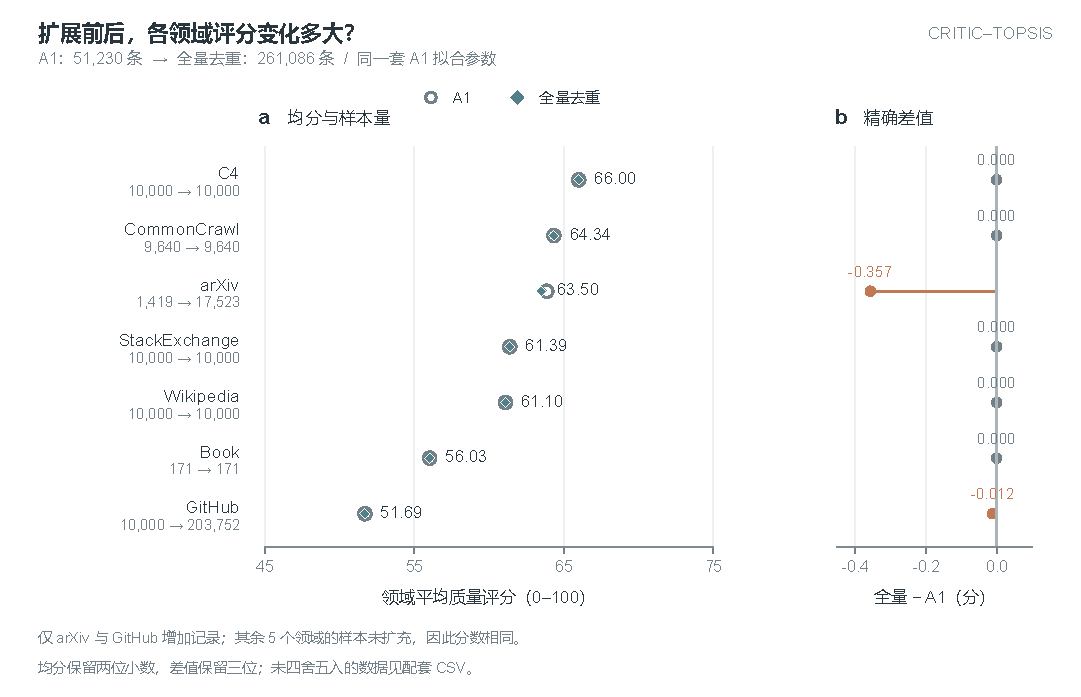
\includegraphics[width=\linewidth]{figures/q1-critic-topsis/nature-v1/figure03_A1_full_comparison_nature.pdf}
  \caption{$A_1$ 抽样集与全量去重语料的质量评分分布及分位点对照。箱线图表示中位数和四分位距，散点表示领域均值。}
  \label{fig:q1-nature-03}
\end{figure}

\paragraph{从样本级到领域级和语料级的聚合}
对领域 $g$ 的记录集合 $\mathcal{I}_g$，采用样本数加权的均值聚合：
\begin{equation}
 Q_g=\frac{1}{|\mathcal{I}_g|}\sum_{i\in\mathcal{I}_g}Q_i,
 \qquad
 Q_{\mathrm{corpus}}=\frac{1}{N}\sum_{i=1}^{N}Q_i.
 \label{eq:q1-domain-aggregation}
\end{equation}
语料级分数即全体唯一记录的算术平均。先评分后聚合的原因在于 TOPSIS 对输入非线性：将领域均值指标重新送入 TOPSIS 后，不等于样本分数的均值。均值聚合保留每条记录的等贡献原则，并将域级差异与域规模分离；中位数与四分位距作为补充统计量在附录报告。

\begin{figure}[htbp]
  \centering
  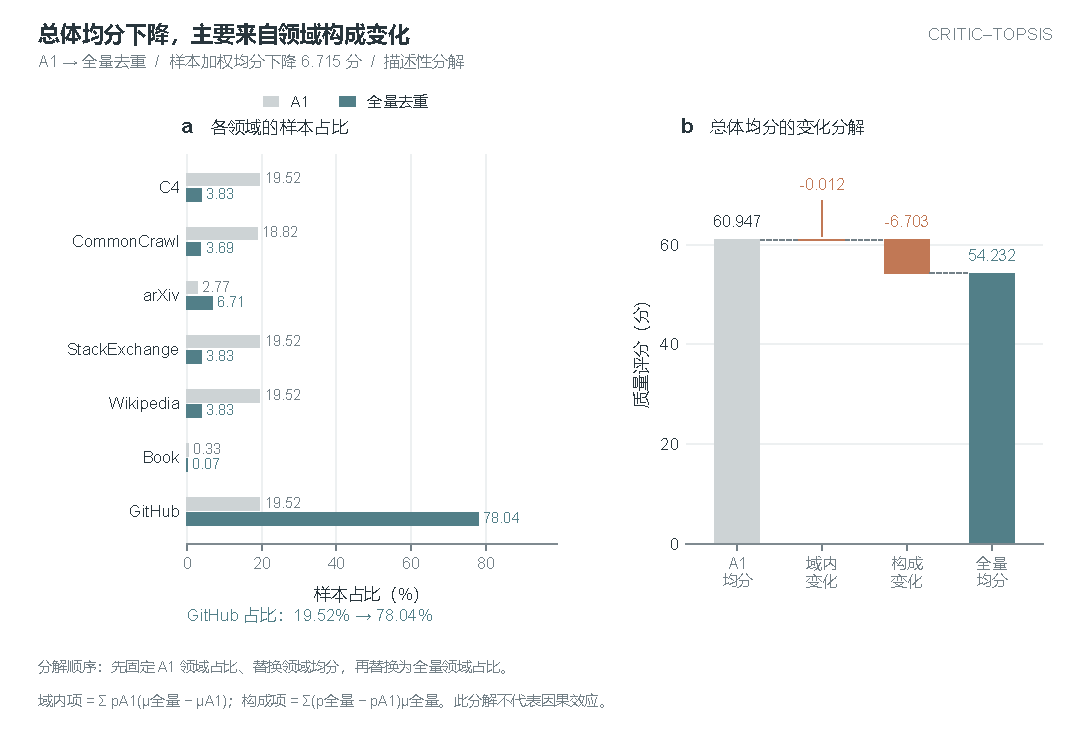
\includegraphics[width=\linewidth]{figures/q1-critic-topsis/nature-v1/figure04_composition_decomposition_nature.pdf}
  \caption{$A_1$ 到全量语料的质量变化分解。总变化分为域内质量变化与领域组成变化两部分。}
  \label{fig:q1-nature-04}
\end{figure}

\paragraph{全量结果与抽样集对照}
$A_1$ 语料级平均分为 $60.95$，全量去重语料平均分为 $54.23$，整体下降 $6.71$ 分。按领域对照：arxiv 从 $63.86$ 变为 $63.51$（下降 $0.36$ 分），github 从 $51.70$ 变为 $51.69$（下降 $0.01$ 分）；book、c4、commoncrawl、stackexchange 和 wikipedia 五个域没有新增记录，领域均值保持不变，不构成独立扩展验证。总体下降主要来自领域组成变化而非域内质量恶化：github 在 $A_1$ 中占 $19.52\%$，在全量语料中占 $78.04\%$，其较低的领域均值显著拉低了语料级分数。按“先替换领域均分、后替换领域占比”的顺序做描述性分解，域内项为 $-0.01$ 分，构成项为 $-6.70$ 分。

\begin{table}[htbp]
  \centering
  \caption{$A_1$ 与全量去重语料的领域级质量分数对照（仅 arxiv、github 两域有新增记录）}
  \label{tab:q1-domain-score}

  \renewcommand{\arraystretch}{1.15}
  \begin{tabular}{lrrrr}
    \toprule
    领域 & $A_1$ 均值 & 全量均值 & 变化 & 全量占比 \\
    \midrule
    arxiv & 63.86 & 63.51 & -0.36 & 6.71\% \\
    github & 51.70 & 51.69 & -0.01 & 78.04\% \\
    book & 56.03 & 56.03 & 0.00 & 3.55\% \\
    c4 & 66.00 & 66.00 & 0.00 & 1.02\% \\
    commoncrawl & 64.34 & 64.34 & 0.00 & 0.92\% \\
    stackexchange & 61.39 & 61.39 & 0.00 & 5.34\% \\
    wikipedia & 61.10 & 61.10 & 0.00 & 4.42\% \\
    \midrule
    语料级均值 & 60.95 & 54.23 & -6.71 & 100.00\% \\
    \bottomrule
  \end{tabular}
\end{table}

\paragraph{稳健性与适用边界}
将 CRITIC--TOPSIS 主方案与等权加权和、删除 DSIR 指标、删除三个负向词组指标三种替代方案比较。主方案与等权结果的 Spearman 秩相关系数为 $0.988$，与删 DSIR 方案为 $0.986$，与删负向指标方案为 $0.967$；在删负向指标方案中平均名次变化 $4.79$ 个百分点，约 $2.78\%$ 的样本名次变化超过 $20$ 个百分点。这表明总分的头部排序对各方案不敏感，但重复性类指标对尾部样本排序有实质影响。该敏感性检验针对的是本小问评分对建模选择的稳定性，它利用的是指标间相关性结构，与本问第二小问所处理的“同一文本上指标评价不一致”是不同概念。

\begin{figure}[htbp]
  \centering
  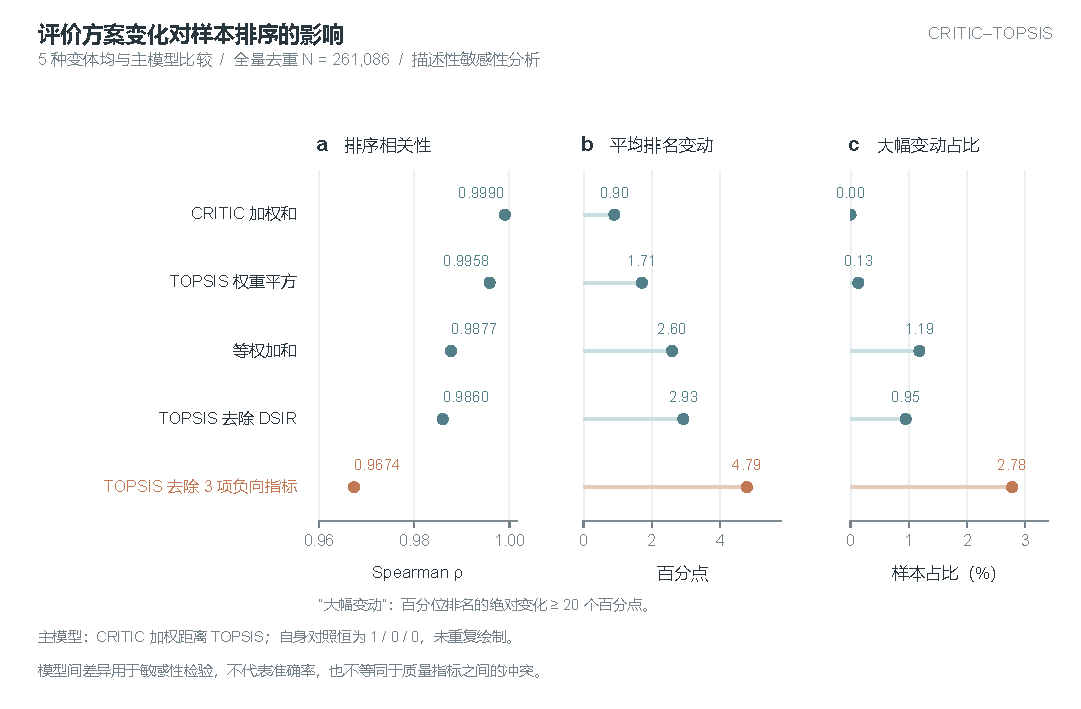
\includegraphics[width=\linewidth]{figures/q1-critic-topsis/nature-v1/figure06_model_sensitivity_nature.pdf}
  \caption{不同权重和指标删减方案下的模型敏感性。左侧展示样本分数的秩相关，右侧展示名次变化及受影响样本比例。}
  \label{fig:q1-nature-06}
\end{figure}

\paragraph{小结}
本小问形成了可复算的全量质量评价链条：以 $A_1$ 稳健边界与 CRITIC 权重建立统一标尺，以加权距离 TOPSIS 输出样本级质量分数，再按记录均值聚合为领域级与语料级分数。结果显示 $A_1$ 与全量语料在已验证域（arxiv、github）的域内质量差异不超过 $0.36$ 分，语料级均分下降的约 $99.8\%$（构成项 $-6.70$ 分，域内项 $-0.01$ 分）由领域构成变化解释。该基线一方面为第二小问的冲突消解提供输入，另一方面输出领域级质量评分 $Q_g$，经 A16 域映射引入后续配比建模与广义标度律，构成四问递进链条的第一环。

% 问题一·第二小问：质量冲突消解（正式章节）
% 由 sections/drafts/q1-conflict-results.tex 清洗接入：移除工作包元话语，统一图号与表述。
% 数据来源：run q1-conflict-*-2026092*（见 experiments/index.csv T-Q1-004）。
\subsubsection{第二小问：质量冲突消解}
\label{sec:q1-conflict}

\paragraph{从单一总分到多维冲突识别}
第一小问的 TOPSIS 总分对 16 个指标采取完全可补偿的聚合：一条“内容价值极高但广告含量高”的文本与一条“各维度均衡中等”的文本可能得到相同的总分。单一总分无法区分这两种结构不同的样本，而题目要求对“不同质量指标对同一文本给出显著不一致评价”的情形单独定义、消解。为此，本小问保留原总分 $Q_i^{(0)}$ 作为基线，回到多维信号层面识别冲突，再构造有限补偿的候选评分作为消解规则。冲突分析覆盖 $A_1$、$A_2$、$A_3$ 全部 $261{,}086$ 条唯一记录，沿用第一小问冻结的归一化与 CRITIC 权重（对原 TOPSIS 领域均分的复算误差小于 $10^{-12}$），并在扩展集上检验主要结论。

\paragraph{五维压缩与冲突定义}
将 16 个通用质量指标按语义压缩为五维，组内继承第一小问权重：
\begin{equation}
z_{ig}=\frac{\sum_{j\in G_g}w_jx_{ij}}{\sum_{j\in G_g}w_j},\qquad
v_g=\frac{\sum_{j\in G_g}w_j}{\sum_h\sum_{j\in G_h}w_j}.
\label{eq:q12-group}
\end{equation}
五维为内容价值、表达质量、整洁度、无广告程度和非重复程度。DSIR 三项与无字母词、句末标点的比例仍保留在原评分和对照试算中，不进入五维模型，该分组是适用性假设而非对这些指标有效性的否定。在 $A_1$ 拟合集上估计各维 $20\%$ 与 $80\%$ 分位数 $l_g=P_{20}(z_g)$、$h_g=P_{80}(z_g)$ 并冻结，定义
\begin{equation}
H_i=\{g:z_{ig}>h_g\},\quad L_i=\{g:z_{ig}<l_g\},\quad
I_i=\mathbf{1}\{H_i\neq\varnothing,\ L_i\neq\varnothing\}.
\label{eq:q12-conflict}
\end{equation}
$I_i=1$ 即判定为候选冲突样本：同一文本同时存在至少一个显著偏高维和至少一个显著偏低维。分位数给出的是相对于拟合分布的偏低或偏高的判断，不是语义缺陷真值，也不是统计显著性检验。按 $H_i$、$L_i$ 是否为空可将全部样本划分为四个互斥且穷尽的类别。进一步定义冲突强度与广度
\begin{equation}
C_i=\max_g\Big[\frac{z_{ig}-h_g}{1-h_g}\Big]_+ + \max_g\Big[\frac{l_g-z_{ig}}{l_g}\Big]_+,
\qquad
B_i=\frac{|H_i|\,|L_i|}{\binom{5}{2}},
\label{eq:q12-strength}
\end{equation}
其中 $[\,\cdot\,]_+$ 表示取正部；由于同一维度无法同时落入高低两端，故而 $C_i$ 的两项不是同一维。

\begin{table}[htbp]
  \centering
  \caption{五维阈值与组权重（由 $A_1$ 拟合集估计并冻结）}
  \label{tab:q1-conflict-thresholds}
  \renewcommand{\arraystretch}{1.15}
  \begin{tabular}{lrrr}
    \toprule
    维度 & 低阈值 & 高阈值 & 组权重 \\
    \midrule
    内容价值 & 0.2783 & 0.5613 & 0.2499 \\
    表达质量 & 0.3578 & 0.7702 & 0.2836 \\
    整洁度 & 0.2673 & 0.9884 & 0.1090 \\
    无广告程度 & 0.5244 & 0.9004 & 0.1056 \\
    非重复程度 & 0.6366 & 0.7838 & 0.2519 \\
    \bottomrule
  \end{tabular}
\end{table}

\paragraph{成因分析}
冲突的候选成因包括：同属性测量分歧（两种教育价值评分器一高一低，$A_1$ 中 415 条、全量去重中 1,402 条）、跨属性权衡（如教育产品推广可同时具有高内容价值与广告属性）、尺度与方向适用性（法律机构名称的必要复述可能触发重复性代理；非英语文本可能被英语流畅度拉低）、同源重复与领域构成变化。基于 15 个定向文本案例的机制分析只能说明存在候选机制，不能估计误判率或证明因果关系。分类器分歧与属性权衡可能存在重叠，不能直接相加计数。

\paragraph{有限补偿综合评价模型}
消解规则的设计目标是：对同属性测量分歧不武断地选择某个评分器，对跨属性权衡引入有界补偿。保留原评分 $Q_i^{(0)}$ 的同时，构造偏好权重的不确定集
\begin{equation}
\mathcal{W}_\lambda=\{(1-\lambda)v+\lambda p:\ p\ge0,\ \textstyle\sum_g p_g=1\},\qquad
Q_i^{\mathrm{cand}}=100\min_{a\in\mathcal{W}_\lambda}\sum_g a_gz_{ig}.
\label{eq:q12-robust}
\end{equation}
即以五维基线权重 $v$ 为中心、允许偏好向量在单纯形内偏离的最坏情形评分。令 $M_i=\sum_gv_gz_{ig}$、$m_i=\min_gz_{ig}$；线性目标在单纯形顶点处取得最小值，故式~\eqref{eq:q12-robust} 有闭式解
\begin{equation}
Q_i^{\mathrm{cand}}(\lambda)=100\big[(1-\lambda)M_i+\lambda m_i\big],\qquad
Q_i^{\mathrm{cand}}-100M_i=-100\lambda(M_i-m_i).
\label{eq:q12-closed}
\end{equation}
当 $0\le\lambda\le1$ 时，候选分位于 $[100m_i,\,100M_i]$ 内且对每一维取值不单调减；各维取值相同为 $c$ 时候选分恰为 $100c$。该规则连续作用于全部样本，不因离散冲突标签跨阈而产生突跳式扣分。$\lambda$ 刻画补偿的有界程度：$\lambda=0$ 退化为完全可补偿的加权均值，$\lambda=1$ 退化为五维最小值（完全不可补偿）。本文取 $\lambda=0.25$ 为主展示值，并比较 $\lambda\in\{0,0.1,0.25,0.5\}$ 的响应；在无外部效度证据前，不认定某一 $\lambda$ 是最优。

\paragraph{结果与扩展检验}
\begin{table}[htbp]
  \centering
  \caption{候选冲突的分层统计（阈值由 $A_1$ 拟合集冻结）}
  \label{tab:q1-conflict-coverage}
  \renewcommand{\arraystretch}{1.15}
  \begin{tabular}{lrrr}
    \toprule
    分区 & 样本数 & 候选冲突数 & 候选冲突率\% \\
    \midrule
    $A_1$ 全量 & 51,230 & 15,124 & 29.52 \\
    $A_1$ 留出 & 10,311 & 3,039 & 29.47 \\
    $A_2$ 重叠 & 1,419 & 798 & 56.24 \\
    $A_2$ 新增 & 16,104 & 9,408 & 58.42 \\
    $A_3$ 重叠 & 10,000 & 3,347 & 33.47 \\
    $A_3$ 新增 & 193,752 & 65,795 & 33.96 \\
    全量去重 & 261,086 & 90,327 & 34.60 \\
    \bottomrule
  \end{tabular}
\end{table}

$A_1$ 中四个类别样本数依次为 15,124、14,958、14,439、6,709，其中第一类即候选冲突类，占比 $29.52\%$，留出集为 $29.47\%$，一致性较好。分域看，arxiv 在 $A_1$ 中的候选冲突率为 $56.24\%$，其新增记录为 $58.42\%$；github 分别为 $33.47\%$ 与 $33.96\%$——两个唯一有新增记录的域上，扩展前后冲突水平接近，主要结论在扩展集上成立；其余五域没有扩展数据，构成不了独立验证。全量冲突率 $34.60\%$ 按 $A_1$ 领域比例重加权后为 $29.67\%$，总体增幅主要来自领域构成变化而非域内冲突水平变化。

\begin{figure}[htbp]
  \centering
  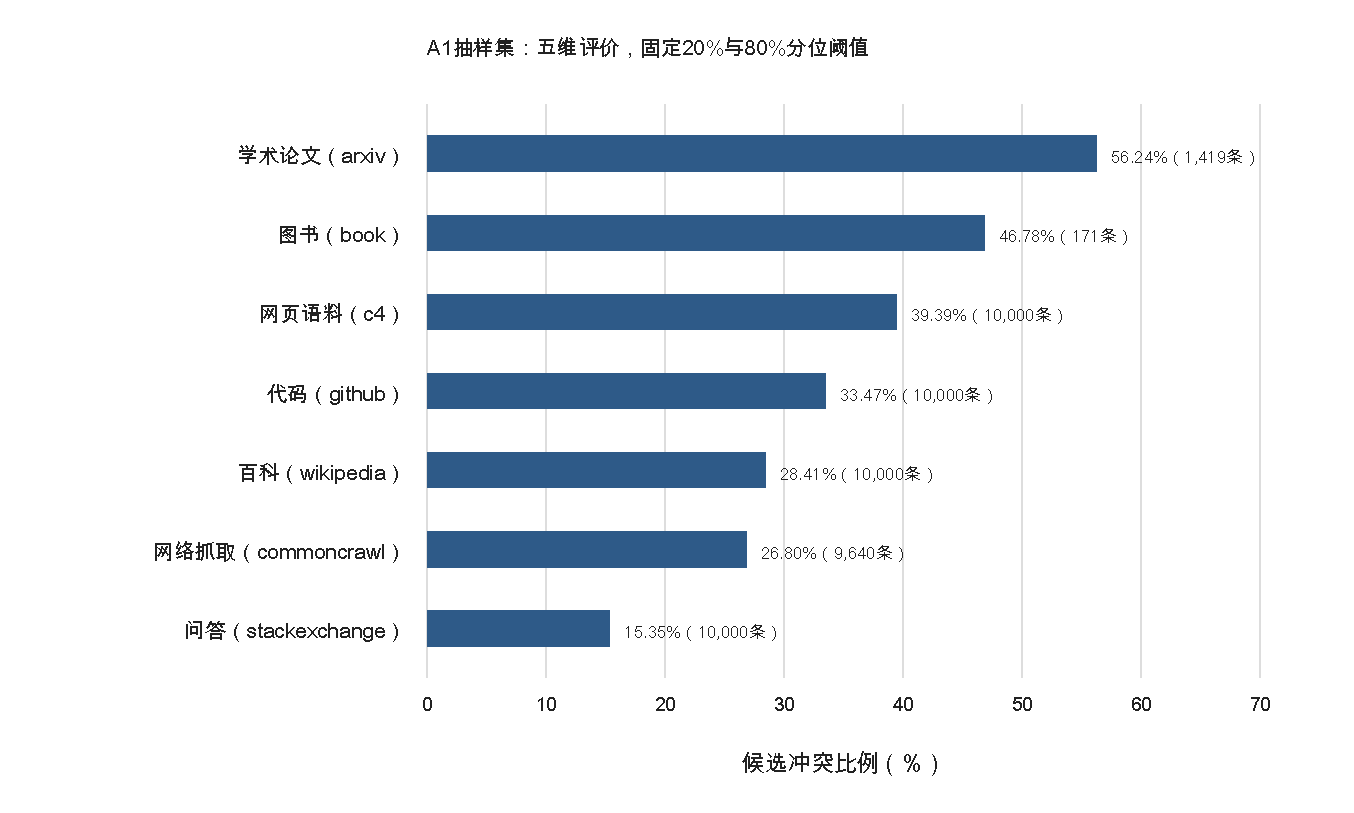
\includegraphics[width=.95\linewidth]{figures/fig1_domain_conflict.pdf}
  \caption{$A_1$ 七域候选冲突率及样本量，阈值由 $A_1$ 拟合集冻结。}
  \label{fig:q1-conflict-01}
\end{figure}

\begin{table}[htbp]
  \centering
  \caption{有限补偿候选评分（$\lambda=0.25$）}
  \label{tab:q1-conflict-resolution}
  \renewcommand{\arraystretch}{1.15}
  \begin{tabular}{lrrrr}
    \toprule
    分区 & 原TOPSIS均分 & 五维加权均分 & 候选稳健均分 & 相对五维基线变化 \\
    \midrule
    $A_1$ 全量 & 60.95 & 58.69 & 52.82 & -5.87 \\
    $A_1$ 留出 & 61.04 & 58.75 & 52.86 & -5.89 \\
    $A_2$ 新增 & 63.47 & 76.54 & 72.25 & -4.29 \\
    $A_3$ 新增 & 51.69 & 46.93 & 40.43 & -6.50 \\
    全量去重 & 54.23 & 51.07 & 44.83 & -6.24 \\
    \bottomrule
  \end{tabular}
\end{table}

需要说明，候选分与原 TOPSIS 分的差距同时混入了指标集合（16 维对 5 维）与聚合方式的变化，不能整体归因于补偿参数 $\lambda$；只有“候选分相对五维加权基线”的变化可以归因于 $\lambda$。以 arxiv 新增样本为例，候选分与原分的 Spearman 秩相关为 $0.611$，说明消解规则对排序有实质影响，选择 $\lambda$ 不是无关紧要的细节。得分降低这个变化本身并不意味着评分更准确，其效度主要依赖外部锚定检验（见第~\ref{sec:results} 节的验证清单）。

\begin{figure}[htbp]
  \centering
  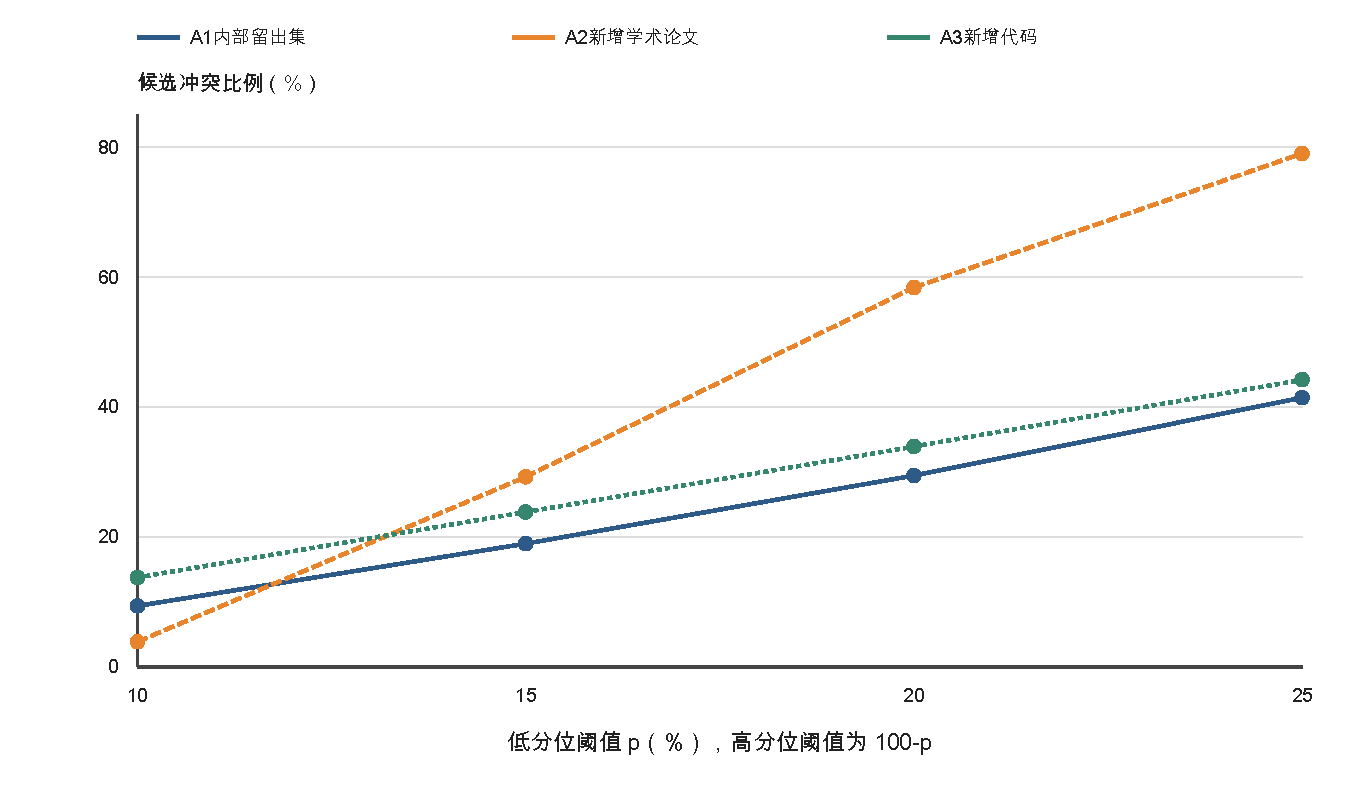
\includegraphics[width=.95\linewidth]{figures/fig2_threshold_sensitivity.pdf}
  \caption{冻结 $A_1$ 拟合参照下的阈值敏感性。}
  \label{fig:q1-conflict-02}
\end{figure}

\paragraph{阈值敏感性与适用边界}
冲突判定对阈值选择敏感：参照分位数由 P10/P90 改为 P25/P75 时，$A_1$ 冲突率由 $9.09\%$ 升至 $41.23\%$，arxiv 新增由 $3.89\%$ 升至 $79.07\%$，且域间相对排序改变。因此本文不以单一阈值的冲突率作为稳健结论，而将其作为随阈值单调响应的描述性量，主结果（扩展前后一致性、构成变化解释）在两种阈值下均成立。一个方向性的交叉检验支持阈值定义的合理性：按“高内容价值且相对低无广告”口径，$A_1$ 有 1,884 条；若改用更严格的“广告 logit 大于无广告 logit”原始口径则仅 310 条，说明相对分位口径捕捉的主要是轻度广告倾向而非强广告文本。

\begin{figure}[htbp]
  \centering
  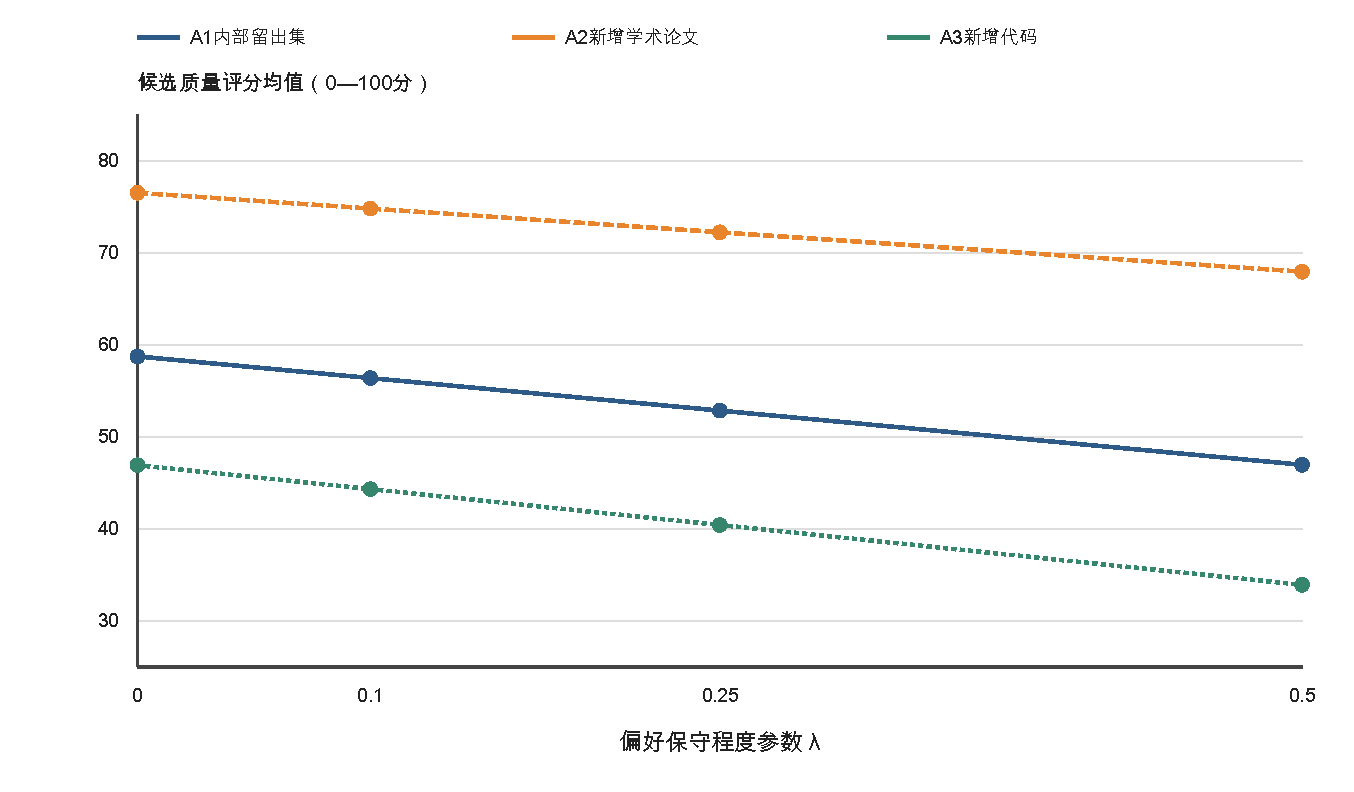
\includegraphics[width=.95\linewidth]{figures/fig3_compensation_sensitivity.pdf}
  \caption{补偿参数 $\lambda$ 对候选均分的影响。}
  \label{fig:q1-conflict-03}
\end{figure}

本小问的适用边界如下。第一，五维分组与冻结分位数均为建模选择，分组方案会主导冲突率水平，本文在固定分组下报告全部结果，分组稳健性分析列为后续工作。第二，目前无人工真值或下游 Loss 证据，候选消解规则的效度尚未外部锚定；据此构造的 83 条分层复核清单仍待标注，正式的 bootstrap 区间与权重扰动检验在本文版本中尚未执行。第三，冲突消解的输出是“带复核标记的候选评分”，不会自动替换第一小问的原评分；原评分继续作为后续三问的输入，候选评分用于敏感性分析。


\subsubsection{第三小问：领域配比建模}
\label{sec:q1-mixture}

本小问利用 RegMix 配方实验数据（A4--A15）建立 17 域配比 $p$ 与交叉熵损失 $L$ 的定量关系。数据按 1M/60M/1B 三个参数尺度组织：A4/A5 为训练集（512 组配方及 13 个验证域损失），A6--A11 为同尺度与跨尺度检验集，A12--A15 为 10B/70B 外推表（配比表与损失表成对使用）。建模需处理三个结构性问题。

第一，\emph{单纯形约束与闭合效应}。配比满足 $p_j\ge0$、$\sum_jp_j=1$，直接在原始坐标上做回归会引入闭合导致的虚假相关；本文以 ilr（等距对数比）坐标变换建立线性模型，并对参考点选择做基敏感性检验。

第二，\emph{尺度条件的必要性}。对 A6/A8 与 A12/A14 中存在的重复配比设计做配对分析发现：更高参数尺度下每一配对目标的损失都更低，且降幅有结构特点——只含配比的模型无法同时表达“同一配比在不同规模下的损失水平”，跨尺度绝对预测在结构上不可辨识。因此本文采用“同尺度建模 + 显式尺度项”的分层方案：同尺度内用 ilr 二次 Ridge 刻画配比的相对结构（五折交叉验证选定正则强度），跨尺度外推仅输出相对排序类结论，不输出绝对损失点预测。该结论在 A10（未见尺度留出）与 A12--A15（外推表）诊断下保持一致的符号方向。

第三，\emph{质量信息的引入}。是否引入第一小问的 $Q_g$ 由数据决定：经 A16 映射，17 个配方域中仅 6 个域可与质量域建立候选关联，其余 11 个域为推断域、无质量锚点。探索性注入实验（6 域质量候选特征）显示质量特征对 1B 留出有所改善，但会恶化 10B/70B 外推表表现，说明在当前数据规模下质量—配比交互的证据不足以进入主模型；主模型保留配比维度，$Q_g$ 经问题二进入标度律。详细的模型比较、共线性审计与逐数据集指标见实验索引（experiments/index.csv 中 T-Q1-003-MIXTURE 系列运行），本节约定的输出为：同尺度配比—损失响应面 $L(p\mid N)$ 及其在检验集上的相对排序精度。
